% compile using this command:
%   pandoc -s -i control_and_systems_synthetic_biology.tex -o control_and_systems_synthetic_biology.html
% "-s" needed to get characters like quotes shown appropriately

% subset of research_for_website_aug2018, extracting as I go; but more edits in this one
% to do by hand:
% center images
%
% 
\documentclass[11pt]{article}

\usepackage{epsf,latexsym,amssymb}
\usepackage{graphicx}

\begin{document}

\section*{Control Systems Theory}

Control theory
%is the area of application-oriented mathematics that
deals with the basic principles underlying the analysis and design of
control systems.  To ``control'' an object means to influence its behavior
so as to achieve a desired goal.  In order to implement this influence,
engineers build devices that incorporate various mathematical techniques.
%%%%%%%%%%%%%%%%%%%%%%%%%%%%%%%%%%%%%%%%%%%%%%%%%%%%%%%%%%%%%%%%%%%%%%%%%%%%
A key enabler of the English Industrial Revolution was Watt's steam engine
fly-ball or centrifugal governor, which built upon Huygens' windmill controller.
%%%%%%%%%%%%%%%%%%%%%%%%%%%%%%%%%%%%%%%%%%%%%%%%%%%%%%%%%%%%%%%%%%%%%%%%%%%%
\medskip

%%%%%%%%%%%%%%%%%%%%%%%%%%%%%%%%%%%%%%%%%%%%%%%%%%%%%%%%%%%%%%%%%%%%%%%%%%%%
\begin{center}
  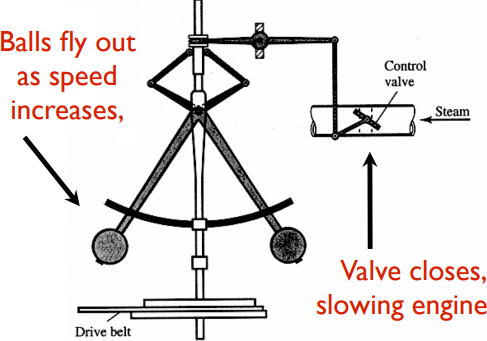
\includegraphics[width=0.2\textwidth]{images/flyball_diagram_from_murray_crop.png}
\end{center}  
%%%%%%%%%%%%%%%%%%%%%%%%%%%%%%%%%%%%%%%%%%%%%%%%%%%%%%%%%%%%%%%%%%%%%%%%%%%%

%  <p><center><img src="images/flyball_diagram_from_murray.png" style="width: 20%;" alt="image" /></center></p>

\medskip

Control systems and feedback play a central role in
aerospace control,
manufacturing,
robotics,
active damping,
climate control of buildings,
chemical process control,
electrical power systems,
consumer products,
active suspensions, automatic braking, engine timing, and self-driving in cars,
mobile communications, power control,
noise cancellation in headphones,
and many other areas of engineering.

\begin{center}
  
\includegraphics[width=0.1125\textwidth]{images/cruise_control.jpg}
  
\includegraphics[width=0.125\textwidth]{images/google_car.jpg}
  
\includegraphics[width=0.037\textwidth]{images/hero-segway_lessqual.jpg}
  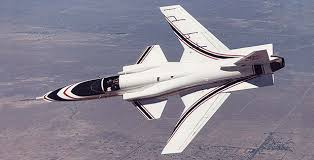
\includegraphics[width=0.1125\textwidth]{images/unstable_airplane_X29.jpg}
  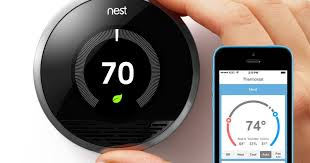
\includegraphics[width=0.1125\textwidth]{images/nest_iphone.jpg}
  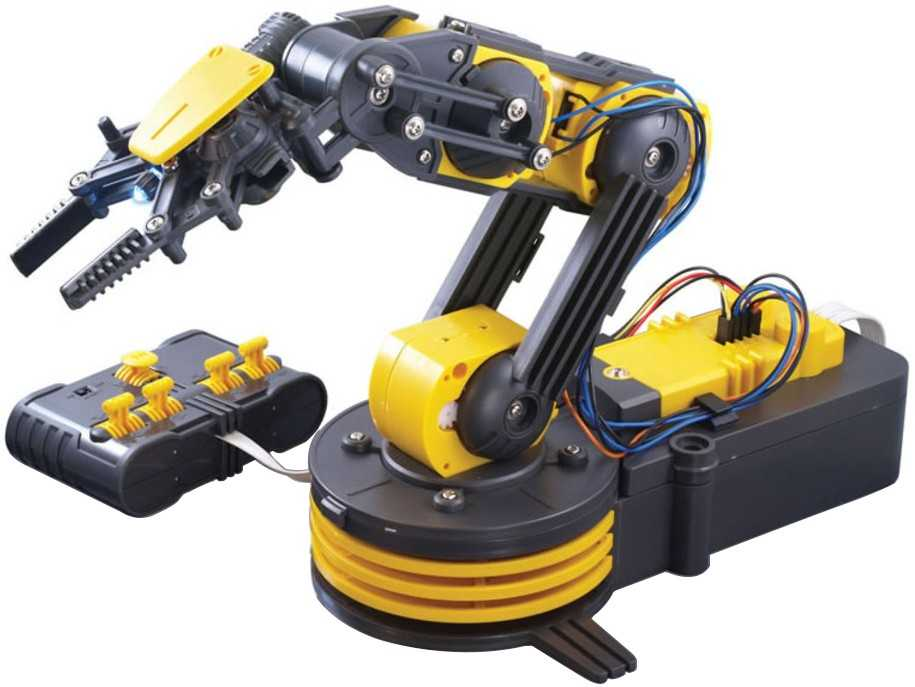
\includegraphics[width=0.1125\textwidth]{images/owi-535-robotic-arm-edge_1_lessqual.jpg}
\end{center}


Control and feedback are also ubiquitous in physiological systems
underlying the homeostatic mechanisms that finely tune internal variables
(such as temperature, pressure, sugar levels, and body fluid balance),
as well as the delicate interplay between infections, tumors, and the immune system.

\medskip

%%%%%%%%%%%%%%%%%%%%%%%%%%%%%%%%%%%%%%%%%%%%%%%%%%%%%%%%%%%%%%%%%%%%%%%%%%%%
\begin{center}
  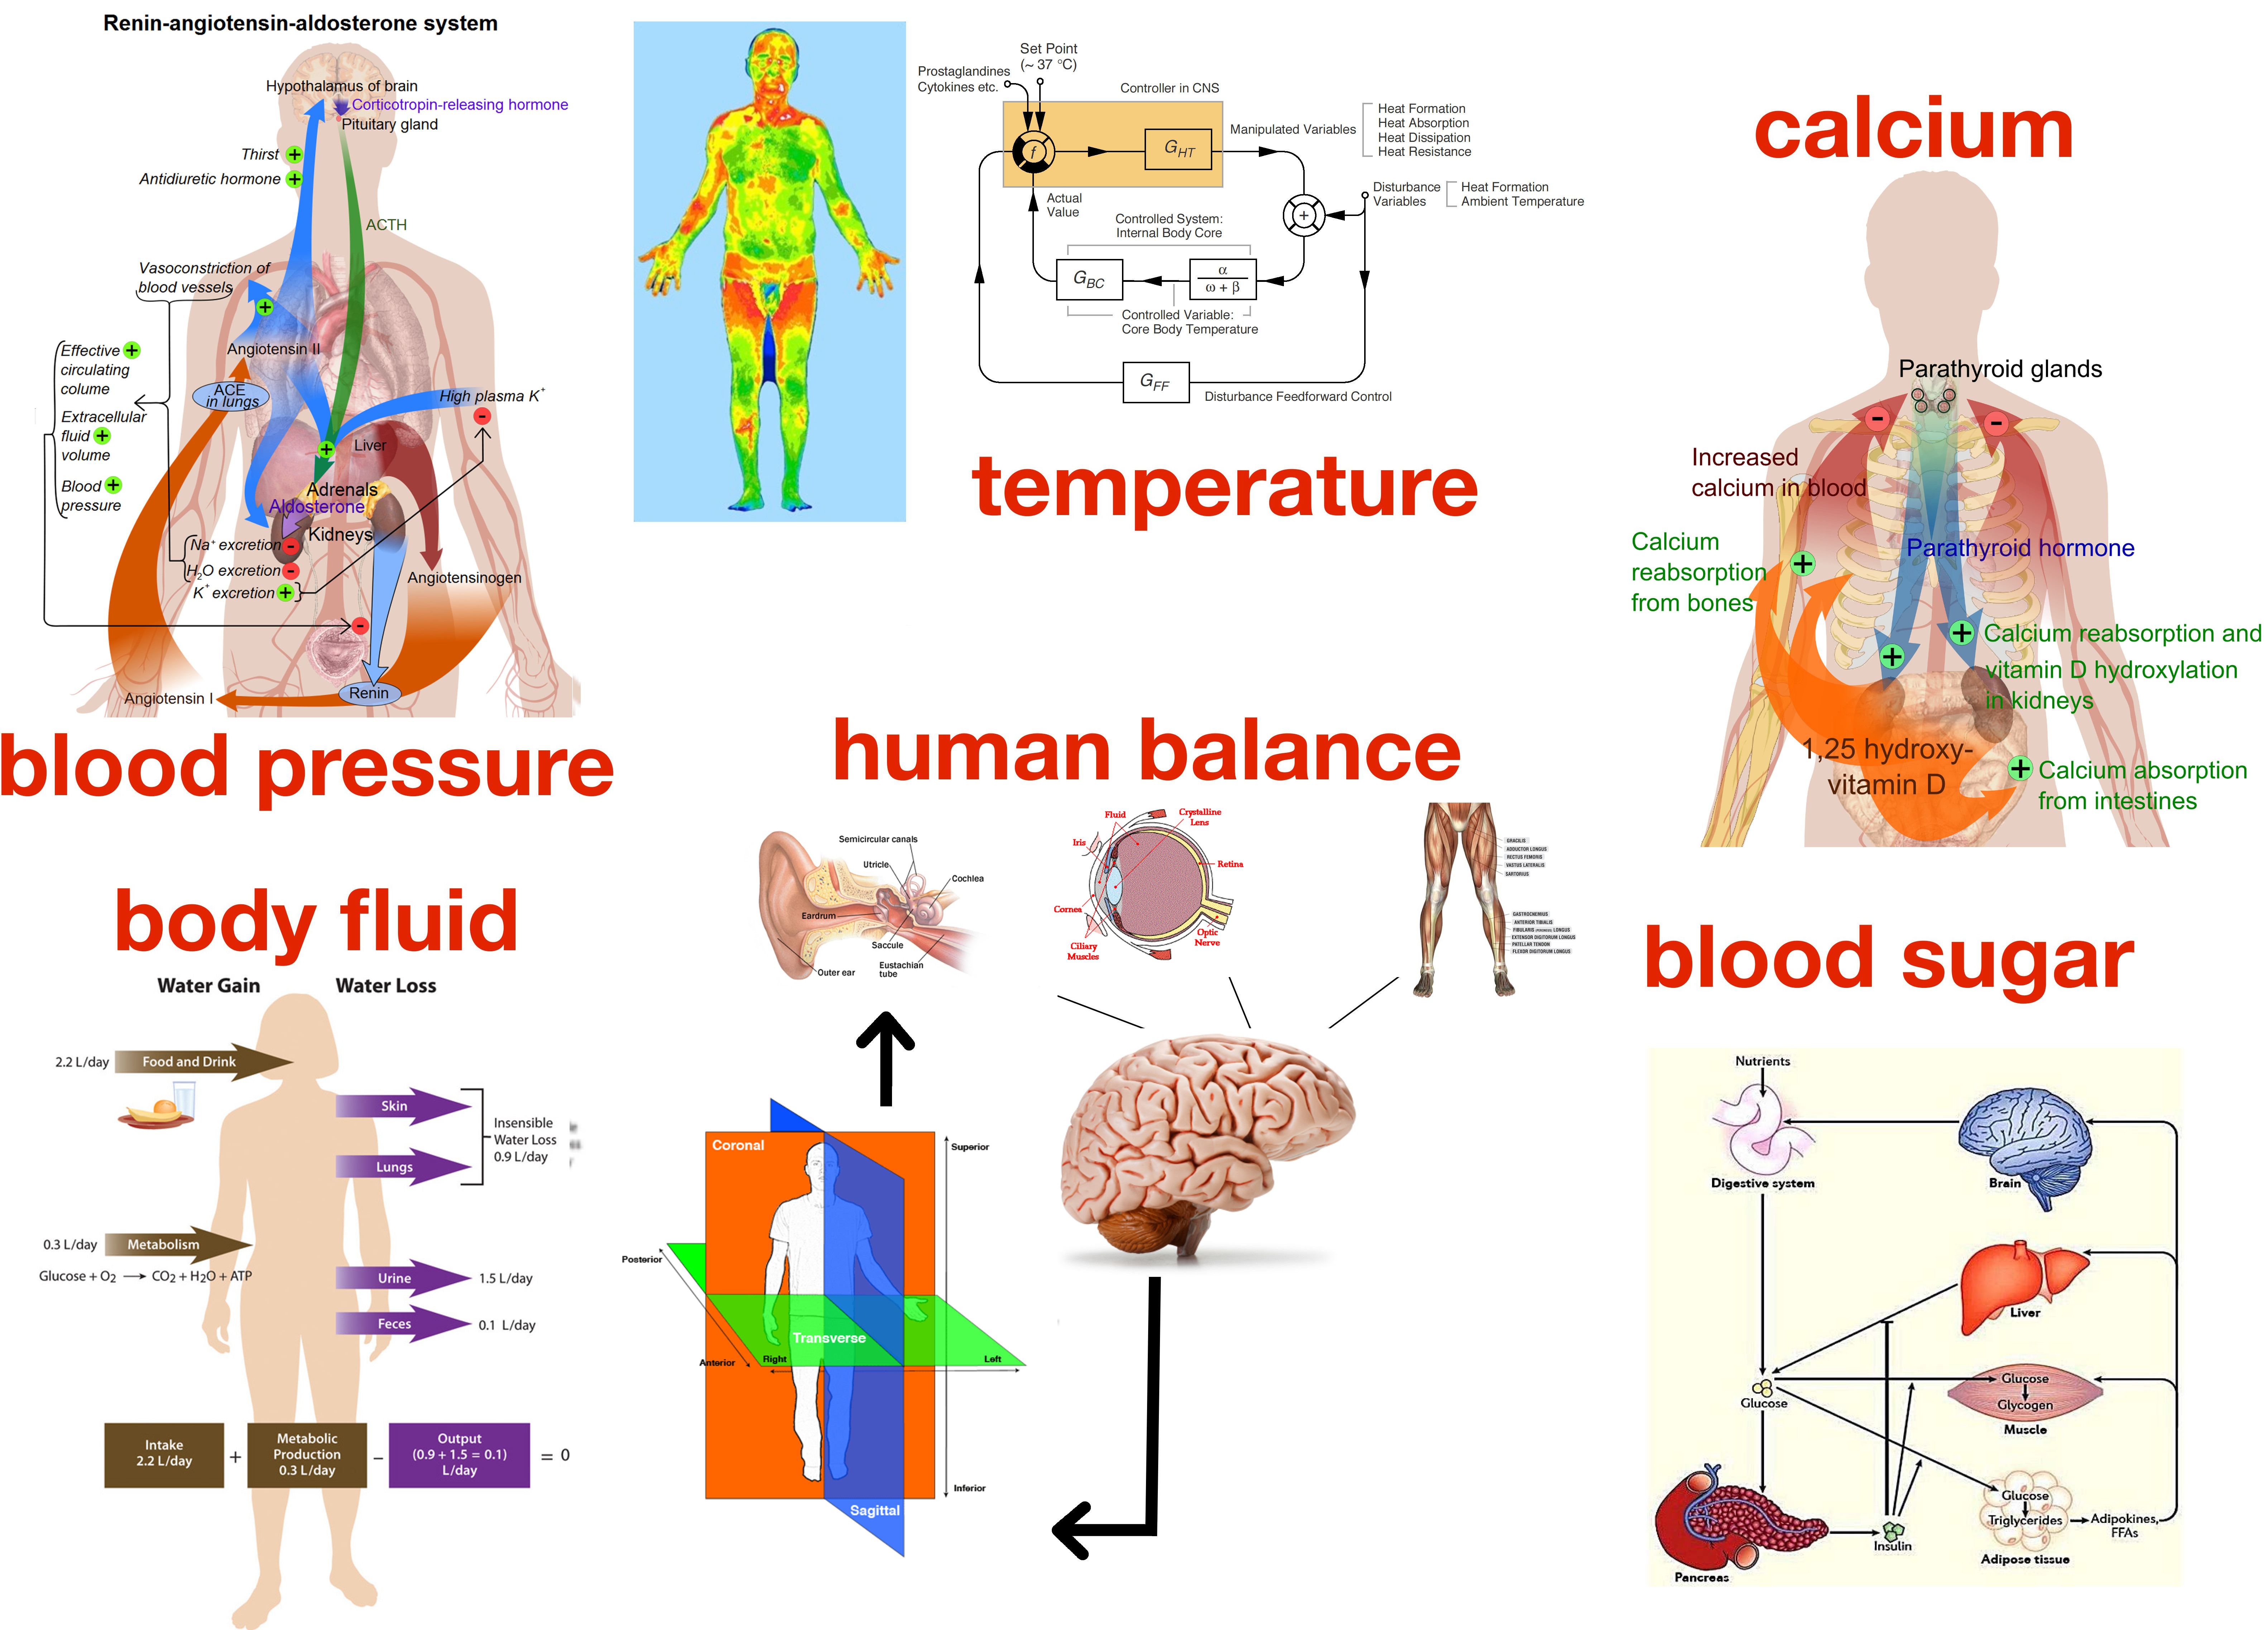
\includegraphics[width=0.5\textwidth]{images/khammash_slides_feedback_control_biology_rearrange_use_better_figs.jpg}
\end{center}  
%%%%%%%%%%%%%%%%%%%%%%%%%%%%%%%%%%%%%%%%%%%%%%%%%%%%%%%%%%%%%%%%%%%%%%%%%%%%

%  <p><center><img src="images/khammash_slides_feedback_control_biology_rearrange_use_better_figs.jpg" style="width: 30%;" alt="image" /></center></p>


The study of control systems and their interaction with the object being
controlled is the subject of control theory.  While on the one hand one wants to
understand the fundamental limitations that mathematics imposes on what is
achievable, irrespective of the precise technology being used, it is
also true that technology may well influence the type of question to be asked
as well as the choice of mathematical model.
%An example of this is the use of difference rather than differential equations
%when one is interested in digital control.
%%%%%%%%%%%%%%%%%%%%%%%%%%%%%%%%%%%%%%%%%%%%%%%%%%%%%%%%%%%%%%%%%%%%%%%%%%%%
Control Theory theory focuses on the \emph{basic theoretical principles
  underlying the analysis of feedback and the design of control systems}
including questions of information processing, signaling, robustness,
feedback, computation, and dynamical properties.  Control theory differs from
the more classical study of dynamical systems because of its emphasis on
inputs (or controls) and outputs (or measurements).

Roughly speaking, there are two main lines of work in control theory.
%%%%%%%%%%%%%%%%%%%%%%%%%%%%%%%%%%%%%%%%%%%%%%%%%%%%%%%%%%%%%%%%%%%%%%%%%%%%
The first of these, known as ``open-loop'' control, aims to plan a sequence of
control actions in order to achieve an objective, often while simultaneously
minimizing a ``cost'' (or maximizing a ``benefit'') criterion. 
Examples are the use use of physical principles and engineering specifications
in order to calculate that trajectory of a spacecraft which achieves a
transfer from one orbit to another, perhaps minimizing total travel time or
fuel consumption, or the scheduling and dosing of chemotherapy with the
objective of eliminating a tumor while minimizing toxicity to the patient.
%%%%%%%%%%%%%%%%%%%%%%%%%%%%%%%%%%%%%%%%%%%%%%%%%%%%%%%%%%%%%%%%%%%%%%%%%%%%
The techniques used in open-loop control are closely related to the classical
calculus of variations and to other areas of optimization theory; the end
result is typically a preprogrammed plan of action (treatment, flight, driving
directions).
%%%%%%%%%%%%%%%%%%%%%%%%%%%%%%%%%%%%%%%%%%%%%%%%%%%%%%%%%%%%%%%%%%%%%%%%%%%%
The second broad line of work is ``feedback'' control, in which rules are
designed so as to correct for deviations from a desired behavior.
Examples include the control systems used during actual space
flight in order to compensate for errors from the precomputed trajectory,
adjustments in therapy to account for patient responses, or GPS-based
navigation systems that use location and road conditions to adjust a
preplanned route. 
%%%%%%%%%%%%%%%%%%%%%%%%%%%%%%%%%%%%%%%%%%%%%%%%%%%%%%%%%%%%%%%%%%%%%%%%%%%%
Feedback helps mitigate the effects of uncertainty in the designer's model of
the object being controlled as well as the environment in which it operates,
and in that sense provides ``robustness'' of control designs.
%%%%%%%%%%%%%%%%%%%%%%%%%%%%%%%%%%%%%%%%%%%%%%%%%%%%%%%%%%%%%%%%%%%%%%%%%%%%
Mathematically, stability theory, dynamical systems, and for linear
systems tools from complex analysis and linear algebra, have had a strong
influence on this approach.
%%%%%%%%%%%%%%%%%%%%%%%%%%%%%%%%%%%%%%%%%%%%%%%%%%%%%%%%%%%%%%%%%%%%%%%%%%%%


\newpage

\section*{Mathematical and Systems Biology}
Now that a map of the human genome is available, one of the most important and
formidable challenges is 
to understand, quantify, and conceptualize the information processing,
regulatory, and dynamic behavior of complex molecular reaction networks
composed of interacting genes, coding and non-coding mRNA's, proteins, small
molecules, metabolites, and other cellular players.

\medskip

Control and feedback are also key organizing principles
in systems biology at a molecular level.  This is a
conceptual diagram (from Hanahan and Weinberg, Cell, 2000) of some of the
central signaling and gene regulatory pathways in cells, whose disruption lead
to the formation of malignant tumors (shown in red are genes known to be
functionally altered in cancer cells):
\medskip
%%%%%%%%%%%%%%%%%%%%%%%%%%%%%%%%%%%%%%%%%%%%%%%%%%%%%%%%%%%%%%%%%%%%%%%%%%%%
\begin{center}
  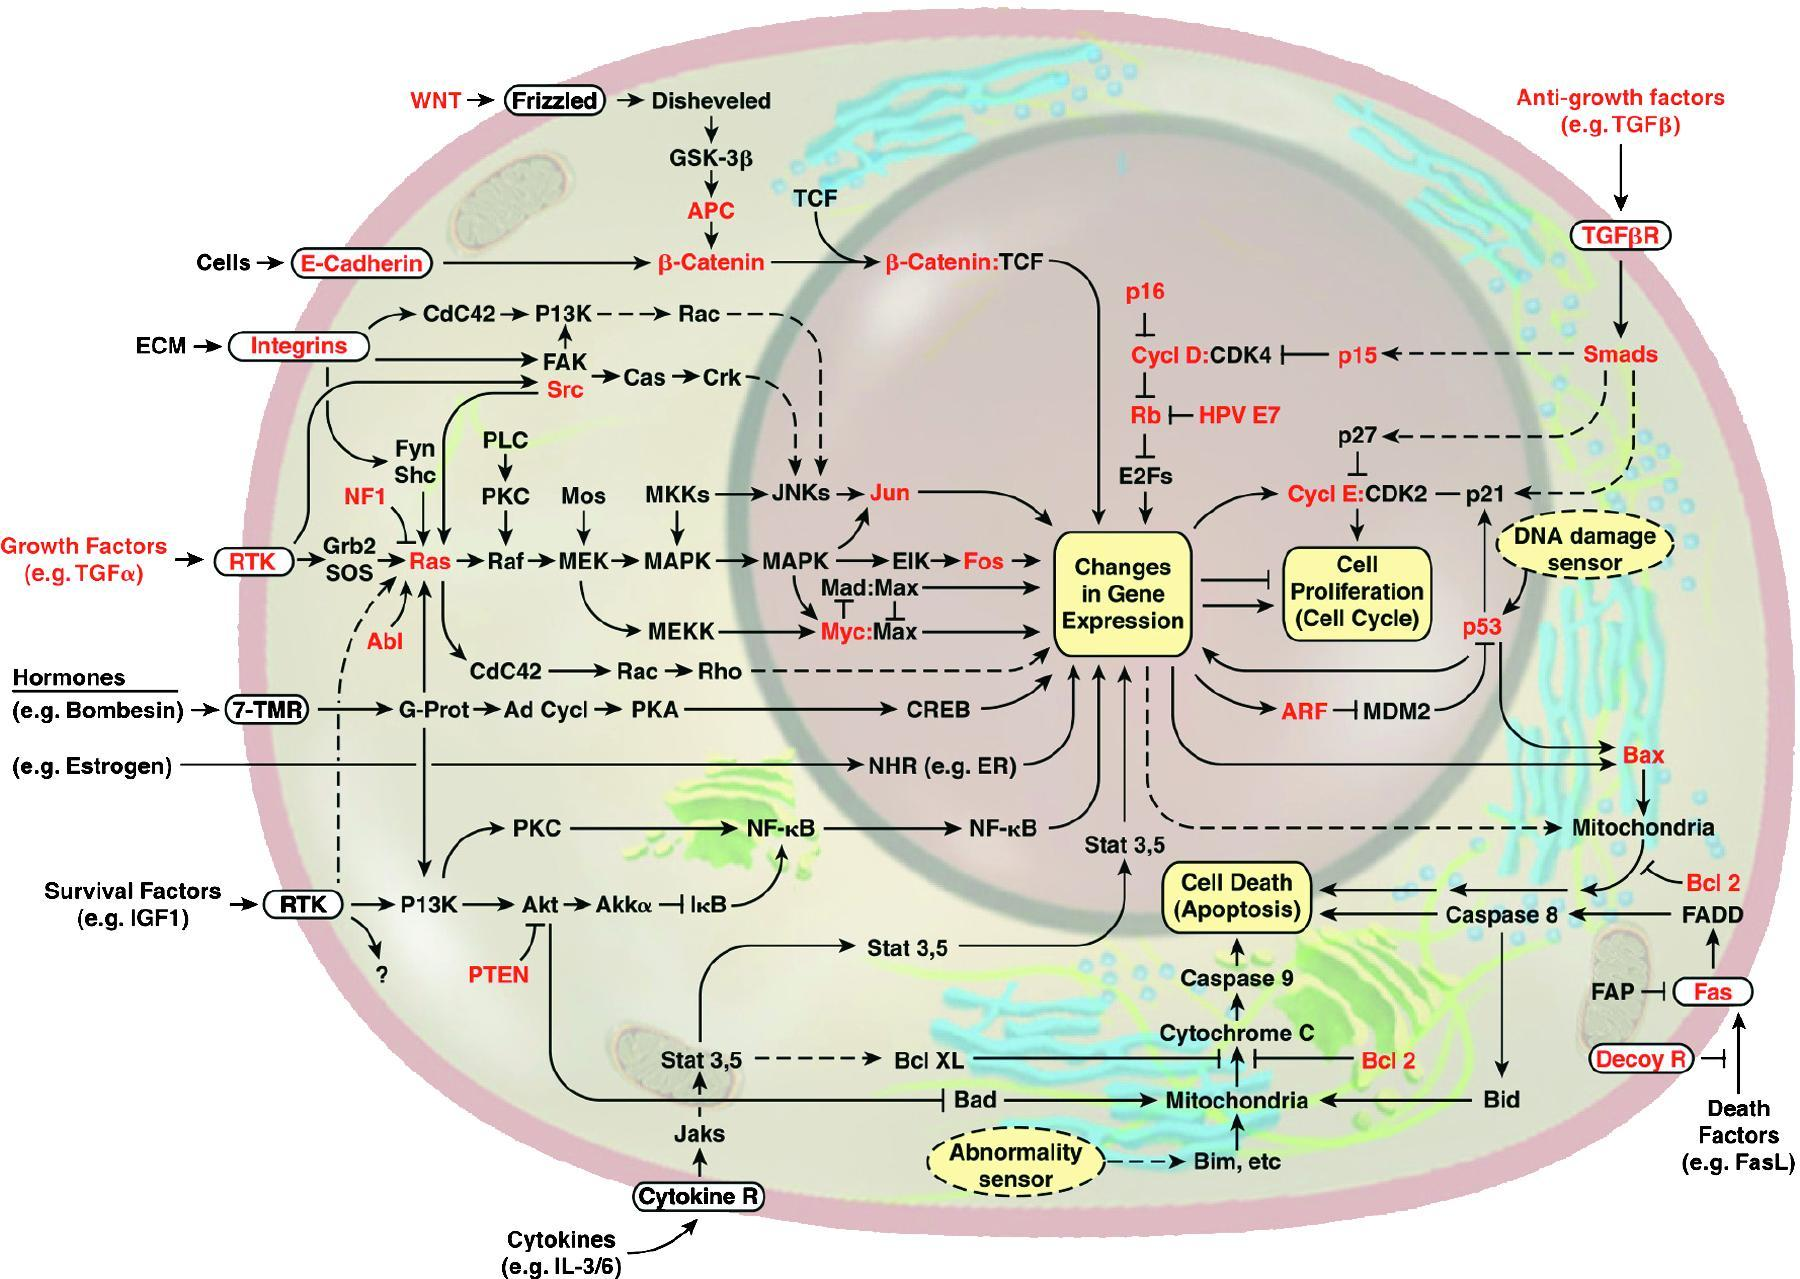
\includegraphics[width=0.4\textwidth]{images/hanahan-weinberg_hihres.jpg}
\end{center} 
%  <p><center><img src="images/hanahan-weinberg_hihres.jpg" style="width: 40%;"alt="image" /></center></p>


%\end{frame}\newsl{3}

When thinking of a diagram like this, one may ask:
What information processing is being performed?
What do the various signaling pathways do?
Why are there feedback and feedforward loops?
What dynamical properties emerge, such as stability or oscillations?
What interventions can be used in order to change undesirable behaviors?
A natural way to approach such problems is afforded by the formalism of
control theory of open systems subject to chemical and physical inputs from
the environment, internal states which describe chemical concentrations, and
observables.



%%%%%%%%%%%%%%%%%%%%%%%%%%%%%%%%%%%%%%%%%%%%%%%%%%%%%%%%%%%%%%%%%%%%%%%%
In fact, completely analogous --and often mathematically equivalent--
questions arise at all scales of biological
organization, from cell interactions with other cells and with their
environment, to tissues, to interactions among immune system
subpopulations, or immune system components with tumors and infectious agents,
to organisms, to embryonic development, and even to full ecosystems.
The mathematics of feedback systems is a universal language, and
conceptually similar ideas underlie the modeling of predator-prey systems
in ecology or in immune/tumor interactions.

\begin{figure}[h]
  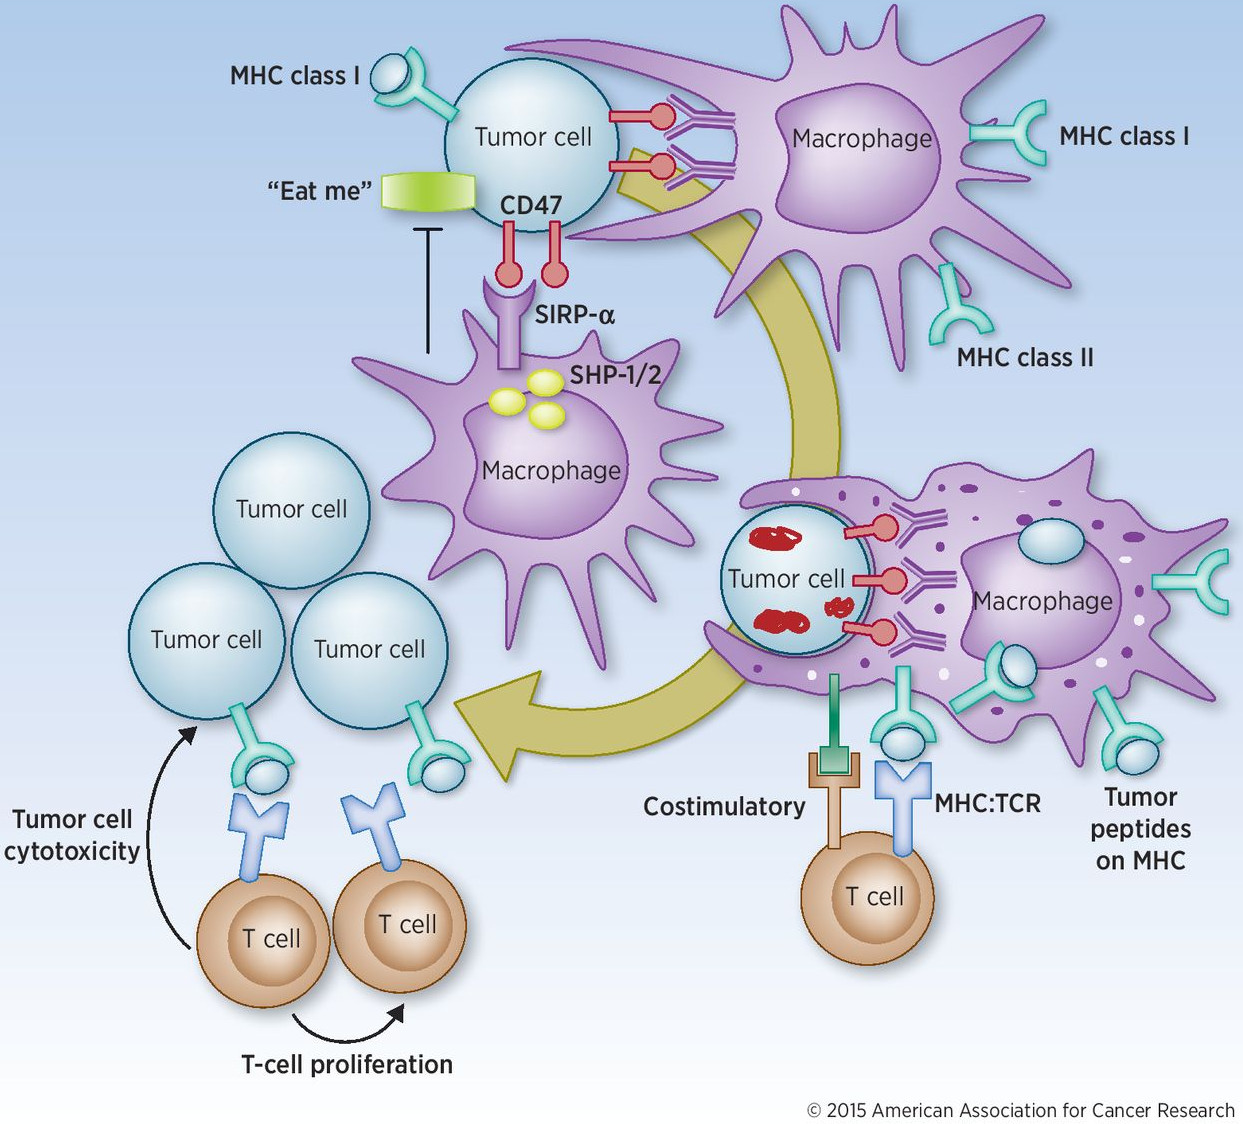
\includegraphics[width=0.2\textwidth]{images/tumor_Tcell_macrophages_from_AACR2015.jpg}
  
\includegraphics[width=0.282\textwidth]{images/lynx_catch_hare_crop.jpg}
\end{figure}

%%%%%%%%%%%%%%%%%%%%%%%%%%%%%%%%%%%%%%%%%%%%%%%%%%%%%%%%%%%%%%%%%%%%%%%%

Dynamics may be studied through systems of ODEs, in which each distinct
``species'' is, depending on the problem of interest, an organism, tissue,
cell type, bacterium, virus, or biomolecule, and the rate of change of each
component is a function of population sizes, interactions among species, and
external factors; of course, for many problems it is more appropriate to
employ PDEs or agent based models, and to include stochastic effects.
%%%%%%%%%%%%%%%%%%%%%%%%%%%%%%%%%%%%%%%%%%%%%%%%%%%%%%%%%%%%%%%%%%%%%%%%
In response, the field of ``systems biology'' has emerged as
an academic domain for education and research, tying together and subsuming
many aspects of physiology, classical biomathematics,
quantitative pharmacology, and biophysics.  
%%%%%%%%%%%%%%%%%%%%%%%%%%%%%%%%%%%%%%%%%%%%%%%%%%%%%%%%%%%%%%%%%%%%%%%%

The ultimate (and arguably very ambitious) goal of the field to bring unity to
the study of feedback control loops and signal processing mechanisms
underlying life, in the process developing novel and powerful mathematical
theory and tools to analyze systems-level biological behavior.
%%%%%%%%%%%%%%%%%%%%%%%%%%%%%%%%%%%%%%%%%%%%%%%%%%%%%%%%%%%%%%%%%%%%%%%%

%%%%%%%%%%%%%%%%%%%%%%%%%%%%%%%%%%%%%%%%%%%%%%%%%%%%%%%%%%%%%%%%%%%%%%%%
On the other hand, given the central role of feedback and signaling mechanisms
in the control of gene expression, protein synthesis, cell division and
differentiation, development, immune responses, and other life-critical
processes, the dysregulation of these mechanisms is a factor in many human
medical disorders.  Thus, it is not unrealistic to expect that the mathematics
of systems biology will eventually also play an important role in clinical
decision-making, complementing statistical and computational tools.  The
emerging field sometimes referred to as ``quantitative biomedicine'' focuses
on translational aspects of systems biology to therapeutic applications.

\section*{Synthetic biology}
The advent of the field of (molecular, systems) ``synthetic biology'' at the
turn of the 21st Century was motivated by two distinct, but mutually
reinforcing, goals.

\medskip
%%%%%%%%%%%%%%%%%%%%%%%%%%%%%%%%%%%%%%%%%%%%%%%%%%%%%%%%%%%%%%%%%%%%%%%%%%%%
\begin{center}
  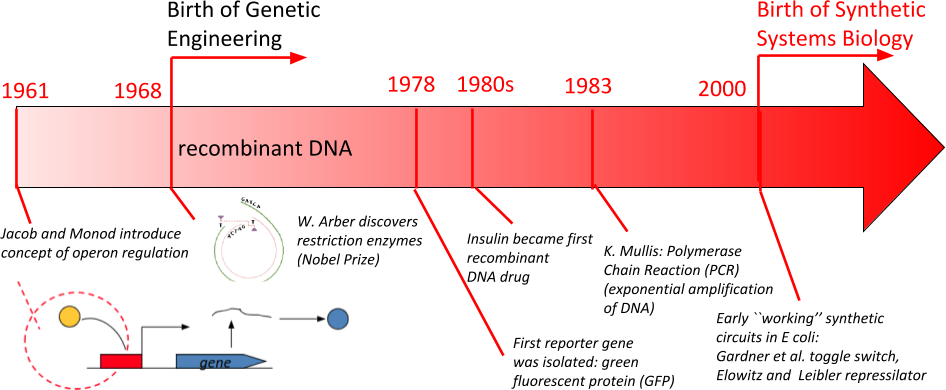
\includegraphics[width=0.4\textwidth]{images/history_synthetic_biology_adapted_from_many_sources_rev1.png}
\end{center} 

A first goal is to design novel --or re-engineer existing-- molecular biological
systems, extending or modifying the 
behavior of organisms, and to control them to perform new tasks.
Through the \emph{de novo} construction of simple elements and circuits, the
field aims to develop a systematic approach to obtaining new cell behaviors in
a predictable and reliable fashion.  
Applications include targeted drug delivery, immunotherapy (e.g., redesign of
cytotoxic T cells to fight tumors), renewable energy (e.g., bio-fuels through
ethanol-producing bacteria), re-engineering bacterial metabolism for waste
recycling, bio-sensing (e.g., detecting environmental pathogens or toxins),
tissue homeostasis (e.g., designing self-differentiating $\beta$ cells in type
1 diabetes treatments), and computing applications (e.g., molecular computing).

A second, and no less important, goal is to improve the
\emph{quantitative and qualitative understanding of basic natural phenomena}.
Experimental validation in theoretical biology is hampered by the practical
difficulties that one faces when attempting to test the validity of models, due
to interlocking regulatory loops in tightly controlled naturally occurring
cellular systems. 
A very useful approach to the testing of (mathematical) models of a biological
system is to \emph{design and construct synthetic versions} of the hypothesized
system (quoting Richard Feymann out of context, ``what I cannot create, I
cannot understand'').
Discrepancies between expected behavior and observed behavior serve to
highlight either research issues that need more studying, or knowledge gaps
and inaccurate assumptions in models.
Synthetic, as opposed to naturally occurring, networks have the advantage that
they can be designed specifically to test hypotheses, thus affording a ``clean
playground'' in which to test models. 
Systems can be built with exactly the components that are believed to be
relevant to a given biological signal processing and/or control function.
In this fashion, the combinatorial effects of multiple feedforward and feedback
loops, or the steps involved in complex cellular responses to stimuli, can be
deconstructed and analyzed.
\emph{The basic knowledge gained from synthetic constructs thus helps advance
our understanding of natural complex systems.}




\end{document}
